\subsection{Sprint 4}

A Sprint 4 foi a última etapa do ReadRace, encerrada com a entrega de 13 de novembro de 2026. Sua preparação combinou funcionalidades ainda previstas com a necessidade de revisar o comportamento da aplicação integrada. O planejamento herdado da sprint anterior incluía a distribuição do aplicativo Android com login, os ajustes nas recompensas de leitura e nos desafios semanais e mensais, além da evolução dos fluxos sociais, da biblioteca e da documentação. Minha participação envolveu testes, correções, revisão de código, melhorias de interface e preparação e condução da apresentação final.

Em 30 de outubro, dediquei-me a mapear bugs na versão implantada da aplicação. O trabalho envolveu testar o sistema, documentar os erros encontrados e preparar o desenvolvimento das correções. Essa atividade mudou o foco da minha participação: além de acompanhar funcionalidades isoladas, passei a observar o comportamento do produto integrado. A avaliação de uso foi realizada por nós, os próprios desenvolvedores. Foi ao utilizar o aplicativo que percebi problemas de UX e que a biblioteca tinha uma apresentação pouco atraente e pouco amigável. Essa percepção orientou minha revisão da interface, procurando tornar as informações mais organizadas e as ações de leitura mais fáceis de encontrar.

Em 3 de novembro, dei continuidade a esse trabalho desenvolvendo e testando correções para os bugs encontrados durante a utilização da aplicação. Um exemplo concreto foi integrado pelo \href{https://github.com/ReadRace-AGES/ReadRace/pull/259}{PR \#259}, de minha autoria: corrigi os cards de grupos que perdiam alinhamento no Android e a biblioteca que permanecia desatualizada após registrar leitura ou adicionar livros. A atualização passou a ocorrer ao retornar à tela, preservando os itens já explorados e o conteúdo exibido durante a consulta. Essa tarefa mostrou que uma funcionalidade podia gravar os dados corretamente e, ainda assim, transmitir uma impressão errada ao usuário se a interface não refletisse a alteração.

Em 11 de novembro, atuei na revisão de pull requests e na integração da aplicação com Playwright. Esse trabalho foi integrado pelo \href{https://github.com/ReadRace-AGES/ReadRace/pull/265}{PR \#265}, de minha autoria, relacionado à \href{https://github.com/ReadRace-AGES/ReadRace/issues/233}{issue \#233}. Configurei testes de ponta a ponta para a versão web do aplicativo em dimensões de celular, com API e PostgreSQL reais em ambiente isolado. O PR registra 22 testes aprovados localmente, sem repetição automática, cobrindo fluxos de biblioteca, leitura, busca, comunidades, clubes, desafios e perfil. O roteiro autenticado com Cognito e a execução no CI ainda exigiam validação naquele registro; os testes de navegador também não substituíam a verificação no Android.

Outra contribuição importante foi o \href{https://github.com/ReadRace-AGES/ReadRace/pull/266}{PR \#266}, no qual trabalhei na experiência de uso e na apresentação visual da biblioteca. Dei mais destaque à leitura em andamento, com título, autor, progresso e acesso direto ao registro de páginas, organizei os filtros das listas e tornei a ação de adicionar livro mais visível. Também melhorei os estados vazios e a identificação das obras quando as capas não carregavam. A revisão se estendeu à clareza da busca, à hierarquia de ações do clube e aos rótulos da navegação. Essas mudanças ajudaram a tornar mais compreensíveis funcionalidades que já existiam.

A Figura~\ref{fig:readrace-biblioteca-ux} apresenta a comparação utilizada na entrega final. Na versão anterior, o cabeçalho e as seções de capas ocupavam grande parte da área inicial. Na versão revisada, o livro em andamento passou a reunir identificação, progresso e registro de leitura em destaque. A comparação ilustra mudanças de hierarquia e de acesso às ações; as capturas usam dados e momentos diferentes e não constituem um teste de usabilidade com leitores.

\begin{figure}[H]
    \centering
    \caption{Biblioteca do ReadRace antes e depois da revisão de UX/UI}
    \label{fig:readrace-biblioteca-ux}
    \begin{minipage}{0.45\linewidth}
        \centering
        {\small Antes da revisão}\par\smallskip
        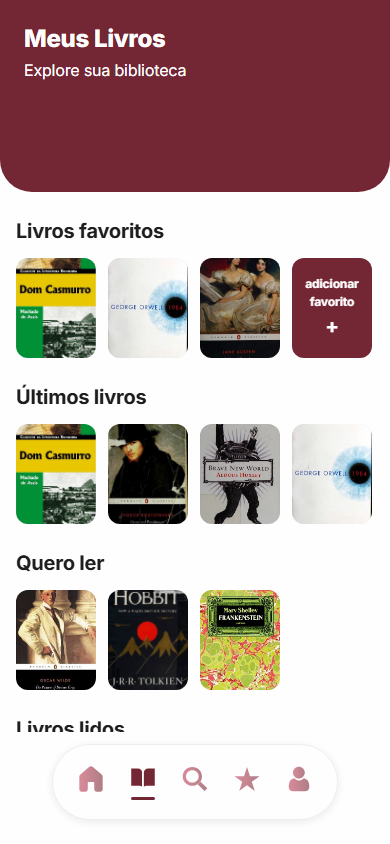
\includegraphics[width=\linewidth,height=0.48\textheight,keepaspectratio]{conteudo/5 - ages IV/conteudo/figures/biblioteca-antes-ui.png}
    \end{minipage}
    \hfill
    \begin{minipage}{0.45\linewidth}
        \centering
        {\small Depois da revisão}\par\smallskip
        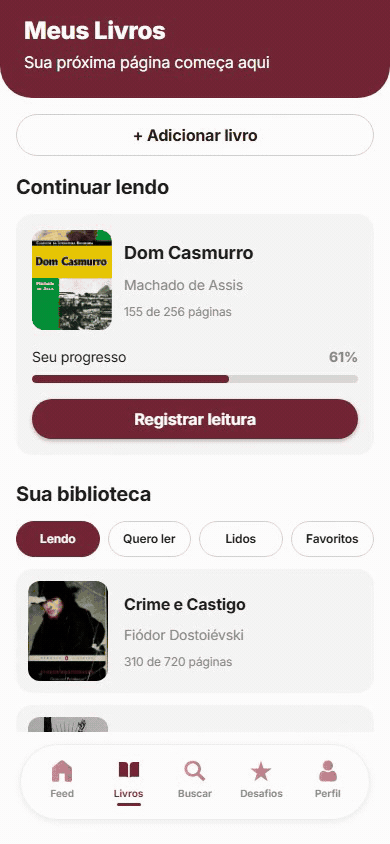
\includegraphics[width=\linewidth,height=0.48\textheight,keepaspectratio]{conteudo/5 - ages IV/conteudo/figures/biblioteca-depois-ui.png}
    \end{minipage}
    \legend{Fonte: apresentação ReadRace --- Sprint 4, Entrega Final, slide 13. Antes: inspeção de 11/11/2026. Depois: quadro extraído da demonstração em GIF.}
\end{figure}

A apresentação final registra 30 testes locais: nove verificações dos fluxos principais, 13 regressões e oito verificações de UX. O material descreve execução com Chromium, API real e PostgreSQL temporário, restaurando os dados entre os testes. Esses números se referem à preparação local da apresentação e complementam os 22 testes descritos inicialmente no PR \#265. As verificações de UX contemplaram telas pequenas, estados vazios e registro direto de leitura. A revisão de interface apresentada foi heurística, sem métricas de avaliação com leitores.

No dia 12 de novembro, trabalhei em correções finais de preparação para a entrega e no desenvolvimento dos slides da apresentação. Na reta final, também implementei a criação de comunidades pelo Feed, integrada pelo \href{https://github.com/ReadRace-AGES/ReadRace/pull/268}{PR \#268}. A funcionalidade inclui formulário, validação, criação conjunta da comunidade e de seu administrador e atualização da lista de comunidades do usuário. A capa é opcional por URL HTTPS; upload de arquivos, edição e transferência de administração ficaram para uma evolução posterior. Também abri o \href{https://github.com/ReadRace-AGES/ReadRace/pull/273}{PR \#273}, que integrou a branch de desenvolvimento à principal no dia da entrega.

No resultado coletivo, algumas pendências das sprints anteriores tiveram seu fechamento registrado no repositório. O \href{https://github.com/ReadRace-AGES/ReadRace/pull/232}{PR \#232} integrou o pagamento de XP dos desafios semanais e mensais; o \href{https://github.com/ReadRace-AGES/ReadRace/pull/254}{PR \#254} passou a apresentar as recompensas logo após o registro de leitura; e o \href{https://github.com/ReadRace-AGES/ReadRace/pull/261}{PR \#261} corrigiu situações que permitiam obter recompensas sem avanço real. A distribuição Android foi tratada no \href{https://github.com/ReadRace-AGES/ReadRace/pull/243}{PR \#243}, que documenta a geração e validação do APK com login contra a API de produção. A disponibilização ocorreu por link de distribuição interna, com Android como plataforma da entrega, sem publicação em loja.

Na demonstração final, organizamos o produto como uma jornada entre Feed, Meus Livros, Busca, Desafios e Perfil. O material apresentou o registro direto de páginas na biblioteca e seu retorno de recompensas, as atividades de leitura das pessoas seguidas, a descoberta e os pedidos de entrada em clubes e a participação em comunidades. Também explicitou os limites do escopo consolidado: iOS, publicação na Play Store, notificações, canal de suporte, enquetes, eventos, recomendações de livros, ranking global e painel administrativo ficaram fora da entrega. Registrar esses cortes ajudava a comunicar com clareza as fronteiras do produto que estava sendo apresentado.

Essas atividades reforçaram minha percepção de que a qualidade de uma entrega depende de um acompanhamento que continua depois da implementação inicial. O mapeamento de bugs, as correções, os testes, a revisão de código e a preparação da apresentação compunham um mesmo esforço de tornar o produto mais consistente e de comunicar seu estado com clareza. Também ficou mais evidente a necessidade de conciliar o tempo dedicado a resolver problemas com a organização das tarefas de encerramento.

Conduzi a apresentação final, assim como havia feito nas Sprints 2 e 3. Esse foi um dos desafios pessoais que estabeleci para a AGES IV: desenvolver minhas soft skills, especialmente a comunicação em apresentações. Preparar os slides, conhecer o estado do produto e explicar o trabalho aos stakeholders me permitiu exercitar essa habilidade de forma recorrente. A evolução da minha participação foi de auxiliar nas primeiras apresentações para assumir a condução das entregas seguintes.

Encerramos o projeto em 13 de novembro com a entrega do que havia sido combinado com os clientes, considerando os ajustes de escopo negociados ao longo do semestre. Eles demonstraram muita satisfação com o resultado e destacaram a diferença percebida entre as Sprints 3 e 4, especialmente as refatorações de UX/UI na biblioteca. Esse retorno foi importante porque mostrou o valor de dedicar esforço à clareza e à organização da experiência de uso, além de ampliar a quantidade de funcionalidades. Também concluímos a documentação de encerramento, incluindo o inventário final do Figma, o registro das diferenças na wiki e os materiais de operação. Esses materiais fizeram parte do fechamento do projeto e da entrega à disposição dos clientes.
